% !TEX root = ../thesis.tex
\documentclass[thesis.tex]{subfiles}
\begin{document}



\chapter{Background}
\label{chapter:background}

T�ss� osassa selvitet��n, mit� tutkimuksen kohteena olevasta aiheesta tiedet��n entuudestaan. Selvityksen tulee kattaa tasapainoisesti koko tutkimuskentt�.

\section{Existing solutions}

There is a wide spectrum of technologies available for product authentication. Applications range from the use of inexpensive seals and electronic labels to carefully crafted watermarks and even DNA. These technologies can be categorized in many ways, for example, by their level of security, cost and portability. The focus of this chapter is on commercial smartphone-based product authentication technologies that often trade high precision (or reliability) for better cost-efficiency and portability. Most of these technologies can be considered as competing solutions for the technology developed in this thesis. Due to the nature of the topic the amount of detailed information on most of the technologies discussed here is limited. An in-depth coverage of different product authentication technologies and their history is given in \cite{kuosmanen}.

\begin{figure}[ht]
\centering 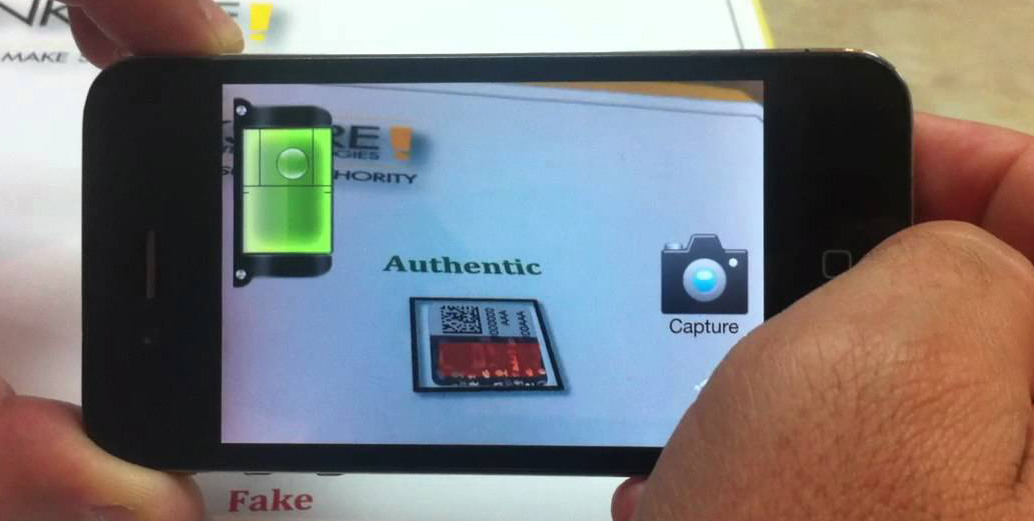
\includegraphics[width=13.25cm]{images/existing_solutions/smartsure}
\caption{InkSure's SmartSure iPhone application UI. The red rectangle and a virtual spirit level are used to position the smartphone correctly. \cite{inksure} \label{figure:inksure}}
\end{figure}

InkSure's SmartSure technology authenticates products by using a chemical marker (taggant) embedded into a hologram. Upon scanning the hologram, the application verifies it based on the presence of the taggant. The taggant is authenticated via a cloud-based platform that also offers track-and-trace reporting services. The application uses a QR scanner and visual aids to help the user position the smartphone's viewfinder properly over the hologram. \cite{inksure} An image of SmartSure's user interface can be seen in Figure \ref{figure:inksure}.

AlpVision offers a technology called CryptoGlyph\textregistered, which uses a pseudo-random pattern of tiny dots (40-80 microns) printed on the coating of the material to authenticate products. The color and size of the dots are customized based on the packaging color. The authenticity of the product is verified by matching the pattern on the product to one stored in a remote database. As of this writing AlpVision's iOS and Android applications are not publicly available in their respective application stores, but instead distributed as tailored applications \textit{``to meet the client's unique authentication needs''}. \cite{alpvision} Figure \ref{figure:alpvision} illustrates how differently sized and color dots affect their visibility and how they are applied to the coating of a material.

\begin{figure}[hb]
\centering 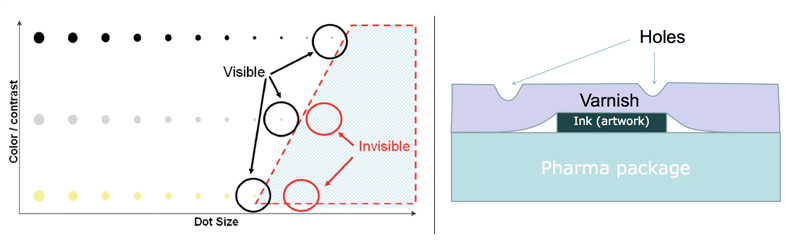
\includegraphics[width=13.25cm]{images/existing_solutions/cryptoglyph}
\caption{AlpVision's CryptoGlyph\textregistered{} embeds micro-dots on the coating of a material to create unique invisible patterns for product authentication \cite{alpvision}. \label{figure:alpvision}}
\end{figure}

The ever growing number of NFC-enabled phones (estimated to reach 53\% of the overall market in 2015 according to \cite{frost-sullivan}) has motivated companies to utilize NFC-based technologies for product authentication. Secure and specialized NFC tags have been manufactured by a number of companies since the technology first hit the market in 2006. However, only few companies have developed the software and services around NFC tags in order to provide end-to-end product authentication. A couple of active players in the field are FinnCode\footnote{\url{http://www.finncode.com/}} and Selinko\footnote{\url{http://selinko.com/}}, which both offer a SaaS-based solution for product authentication and manufacture secure NFC tags.

Other notable technologies built around the capabilities of a smartphone include scryptoTRACE\textregistered{} by U-NICA\footnote{\url{http://www.u-nica.com/1320.html}}, CertiEye by Infotoo Ltd.\footnote{\url{http://www.certieye.com/}} and AuthentiGuard by DSS Inc.\footnote{\url{http://www.authentiguard.com/products.html\#tab_authentiguard}}. A summary of the aforementioned technologies is provided in Table \ref{table:existing-solutions}. Next, Chapter \ref{section:photoluminescence} discusses the theory behind photoluminescence and how it can be applied in product authentication.

\begin{table}[hb]
	\caption{Existing solutions for smartphone-based product authentication.} \label{table:existing-solutions}

	\begin{center}
	\begin{tabular}{| m{2cm} | m{3.25cm} | m{3cm} | m{3.75cm} |}

		\hline
		\textbf{Company}				&	\textbf{Product name}			&	\textbf{Platforms}		&	\textbf{Technologies} \\ \hline
		InkSure\newline (American)		&	SmartSure						&	iPhone					&	- chemical taggant\newline- hologram \\ \hline
		U-NICA\newline (Swiss)			&	scryptoTRACE\textregistered		&	iPhone, Android			&	- micro-printing\newline- edge detection \\ \hline
		AlpVision\newline (Swiss)		&	CryptoGlyph\textregistered		&	Customized*				&	- micro-printing\newline- pattern recognition \\ \hline
		DSS\newline (American)			&	AuthentiGuard					&	Customized*				&	 \\ \hline
		Infotoo\newline (Chinese)		&	CertiEye						&	iPhone, Android			&	 \\ \hline
		FinnCode\newline (Finnish)		&									&	iPhone, Android			&	- NFC \\ \hline
		Selinko\newline (Belgian)		&									&	Android					&	- NFC \\
		\hline
	\end{tabular}
	\end{center}
	\small{* privately distributed, the application is developed according to the client's needs.}
\end{table}

\section{Photoluminescence}
\label{section:photoluminescence}



\section{Mobile Platforms, Tools and Frameworks}
- jni, c++/cx, ios with c++?

\section{Hybrid Applications}

Hybrid applications are essentially small websites running in a browser shell in an application that have access to the native platform layer. Hybrid applications have many benefits over pure native applications, specifically in terms of platform support, speed of development, and access to 3rd party code.

\section{Mobile Camera Technology}

\subsection{Sensors}
\subsection{Pixel Formats}
\subsection{Camera Flash}

\section{RGB and HSV color spaces}

\end{document}